% by pts@fazekas.hu at Fri Aug 28 09:29:30 CEST 2009
%
% !! reorder slides
% !! rename to better reflect not-TeX-only
% !! mark the documents that are by TeX
% !! no colors in the document size chart
% !! add file sizes to the bottom of graph 2
%
% SUXX: pdflatex cannot embed (missing glyph) a Keynote chart with an ff
%       ligature in the caption. Solution: ZERO-WIDH-JOINER unicode char.
\documentclass{beamer}
\usepackage{lmodern}
\usepackage{t1enc}
\usepackage{graphicx}
\usepackage{beamerthemesplit}
\usepackage{color}


\definecolor{GoogleBlue}{RGB}{0,102,204}
\definecolor{GoogleRed}{RGB}{255,0,0}
\definecolor{GoogleYellow}{RGB}{255,204,0}
\definecolor{GoogleGreen}{RGB}{0,153,0}
\RequirePackage{xspace}
\newcommand\Google{% The Googley \Google :)
\texorpdfstring{% Color changes do not like to be in bookmarks.
{\color{GoogleBlue}G}%    G
{\color{GoogleRed}o}%     o
{\color{GoogleYellow}o}%  o    :)
{\color{GoogleBlue}g}%    g
{\color{GoogleGreen}l}%   l
{\color{GoogleRed}e}%     e
}{Google}% Colorless text used instead when colors won't work.
\xspace}

\definecolor{c-purple}{rgb}{0.4353,0.2392,0.4745}
\definecolor{c-red}{rgb}{0.7373,0.1765,0.1882}
\definecolor{c-yellow}{rgb}{0.9059,0.6314,0.2392}
\definecolor{c-green}{rgb}{0.3647,0.5882,0.2824}
\definecolor{c-blue}{rgb}{0.1804,0.3412,0.5490}

\title{Optimizing PDF output size of \TeX{} documents}
\subtitle{\ldots{} and PDF files created by other means as well}
\author[P\'eter Szab\'o]{P\'eter Szab\'o\\\textbf{\Google}}
\date{2009-08-31\par\medskip EuroTeX\,2009\\ The Hague, The Netherlands}

%** Create a colorful full square with the specified color.
\def\colorsquare#1{{\color{#1}\vrule width.8em height.8em depth0pt}}

%** Put content to a frame with raggedbottom vertical alignment.
%** This has a hard-coded height for the useful content, depends on the
%** number of sections as well.
%** @example
%**   \frame{
%**      \nocenterframetitle{...}
%**      \nocenter{
%**      ...
%**      }
%**   }
\def\nocenter#1{%
  \hrule height0pt
  \vbox to200pt{\vsize=200pt{\ignorespaces#1}\vfil}%
}

\begin{document}

\frame{\titlepage}

% !!
\section[Outline]{}
\frame{\tableofcontents}

\section{Optimization effectiveness}

\subsection{Input PDF files}

\frame{
\frametitle{Input PDF files}
\begin{description}
\item[cff] \emph{CFF reference}; 62 pages; by FrameMaker $+$ Distiller
\item[beamer] first beamer.cls example; 75 slide-steps; by pdf\TeX{}
\item[eu2006] proceedings; 126 pages; by pdf\TeX{} $+$ concat
\item[inkscape] Inkscape manual; 341 pages; by CodeMantra
\item[lme2006] proceedings in Hungarian; 240 pages; by dvips $+$ ps2pdf $+$ concat
\item[pdfref] \emph{PDF\,1.7 reference} 1310 pages; by FrameMaker $+$ Distiller
\item[pgf2] \emph{TikZ manual} 560 pages; by pdf\TeX{}
\item[texbook] \emph{The \TeX{}book} 494 pages; by pdf\TeX{}
\item[tuzv] mini novel in Hungarian; 20 pages; by dvipdfm
\end{description}
}

\frame{
\frametitle{Input PDF sizes}
\nocenter{%
%\vbox to 0pt{}%
%\nointerlineskip
\noindent\hfil
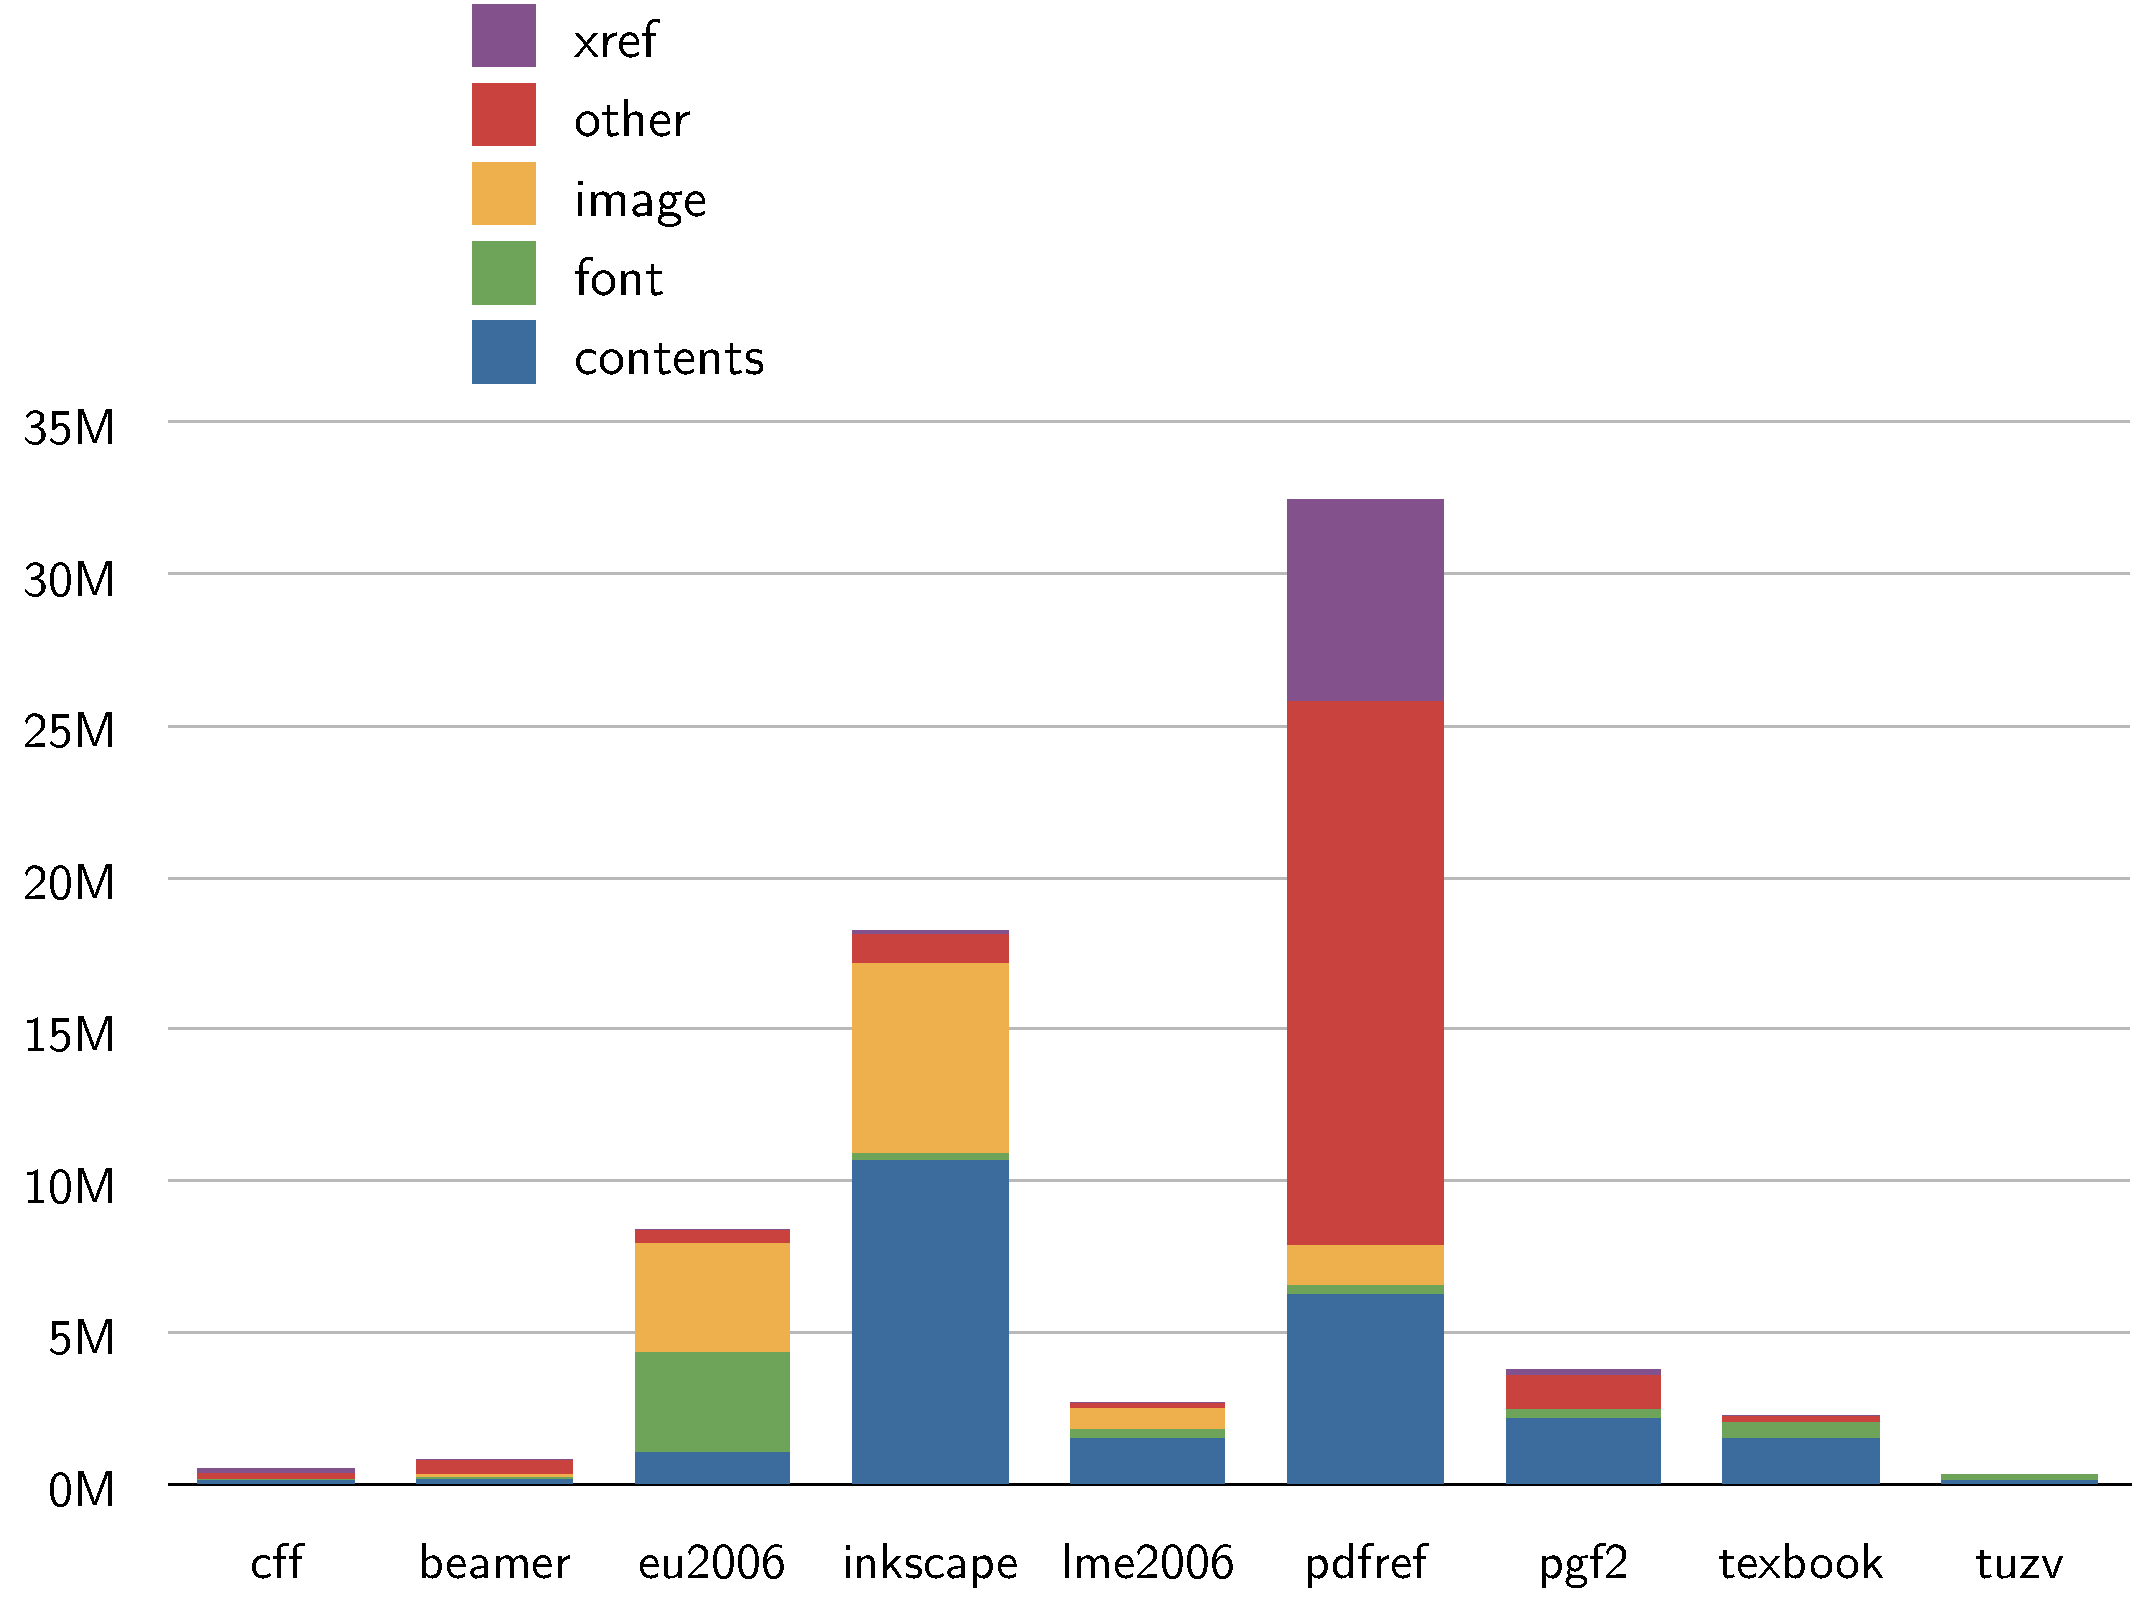
\includegraphics[height=\vsize]{pdfsizeopt_charts.pdf}
}}

\frame{
\frametitle{PDF features measured}
\begin{description}
\item[xref \colorsquare{c-purple}] cross-reference table containing the document offsets
\item[other \colorsquare{c-red}] hyperlinks, anchors, page structure, section structure
(outlines), submittable forms, and other metadata
\item[image \colorsquare{c-yellow}] embedded pixel images (XObject and inline)
\item[font \colorsquare{c-green}] embedded vector font data
\item[contents \colorsquare{c-blue}] vector graphics, text, colors, patterns
etc., including content streams and form XObjects
\end{description}
}

\frame{
\frametitle{Input PDF feature distribution}
\nocenter{%
\noindent\hfil
\includegraphics[height=\vsize,page=2]{pdfsizeopt_charts.pdf}
}}

\subsection{Optimization effectiveness by feature}

%\frame{
%\frametitle{Image optimization effectiveness (byte sizes)}
%\nocenter{%
%\noindent\hfil
%\includegraphics[height=\vsize,page=3]{pdfsizeopt_charts.pdf}
%}}

\frame{
\frametitle{Vector graphics and text optimization effectiveness}
\nocenter{%
\noindent\hfil
\includegraphics[height=\vsize,page=4]{pdfsizeopt_charts.pdf}
}}

\frame{
\frametitle{Embedded font optimization effectiveness}
\nocenter{%
\noindent\hfil
\includegraphics[height=\vsize,page=5]{pdfsizeopt_charts.pdf}
}}

\frame{
\frametitle{Pixel image optimization effectiveness}
\nocenter{%
\noindent\hfil
\includegraphics[height=\vsize,page=6]{pdfsizeopt_charts.pdf}
}}

\frame{
\frametitle{Other data optimization effectiveness}
\nocenter{%
\noindent\hfil
\includegraphics[height=\vsize,page=7]{pdfsizeopt_charts.pdf}
}}

\frame{
\frametitle{Cross-reference optimization effectiveness}
\nocenter{%
\noindent\hfil
\includegraphics[height=\vsize,page=8]{pdfsizeopt_charts.pdf}
}}

\section{Discussion}
%\subsection{Overview of the Beamer Class}
\frame
{
  \frametitle{Features of the Beamer Class}

  \begin{itemize}
  \item<1-> Normal LaTeX class.
  \item<2-> Easy overlays.
  \item<3-> No external programs needed.      
  \end{itemize}
}
\end{document}
